\documentclass[11pt,a4paper]{article}
\usepackage[utf8]{inputenx}
\usepackage[T1]{fontenc}
\usepackage{textcomp}
\usepackage{ marvosym }
\usepackage{pdfpages}
%opening
\title{Progettazione Logica}
\author{Attilio Lughetta N97000\\Giusy Gaudino N97000283}
\date{}
\begin{document}

\maketitle
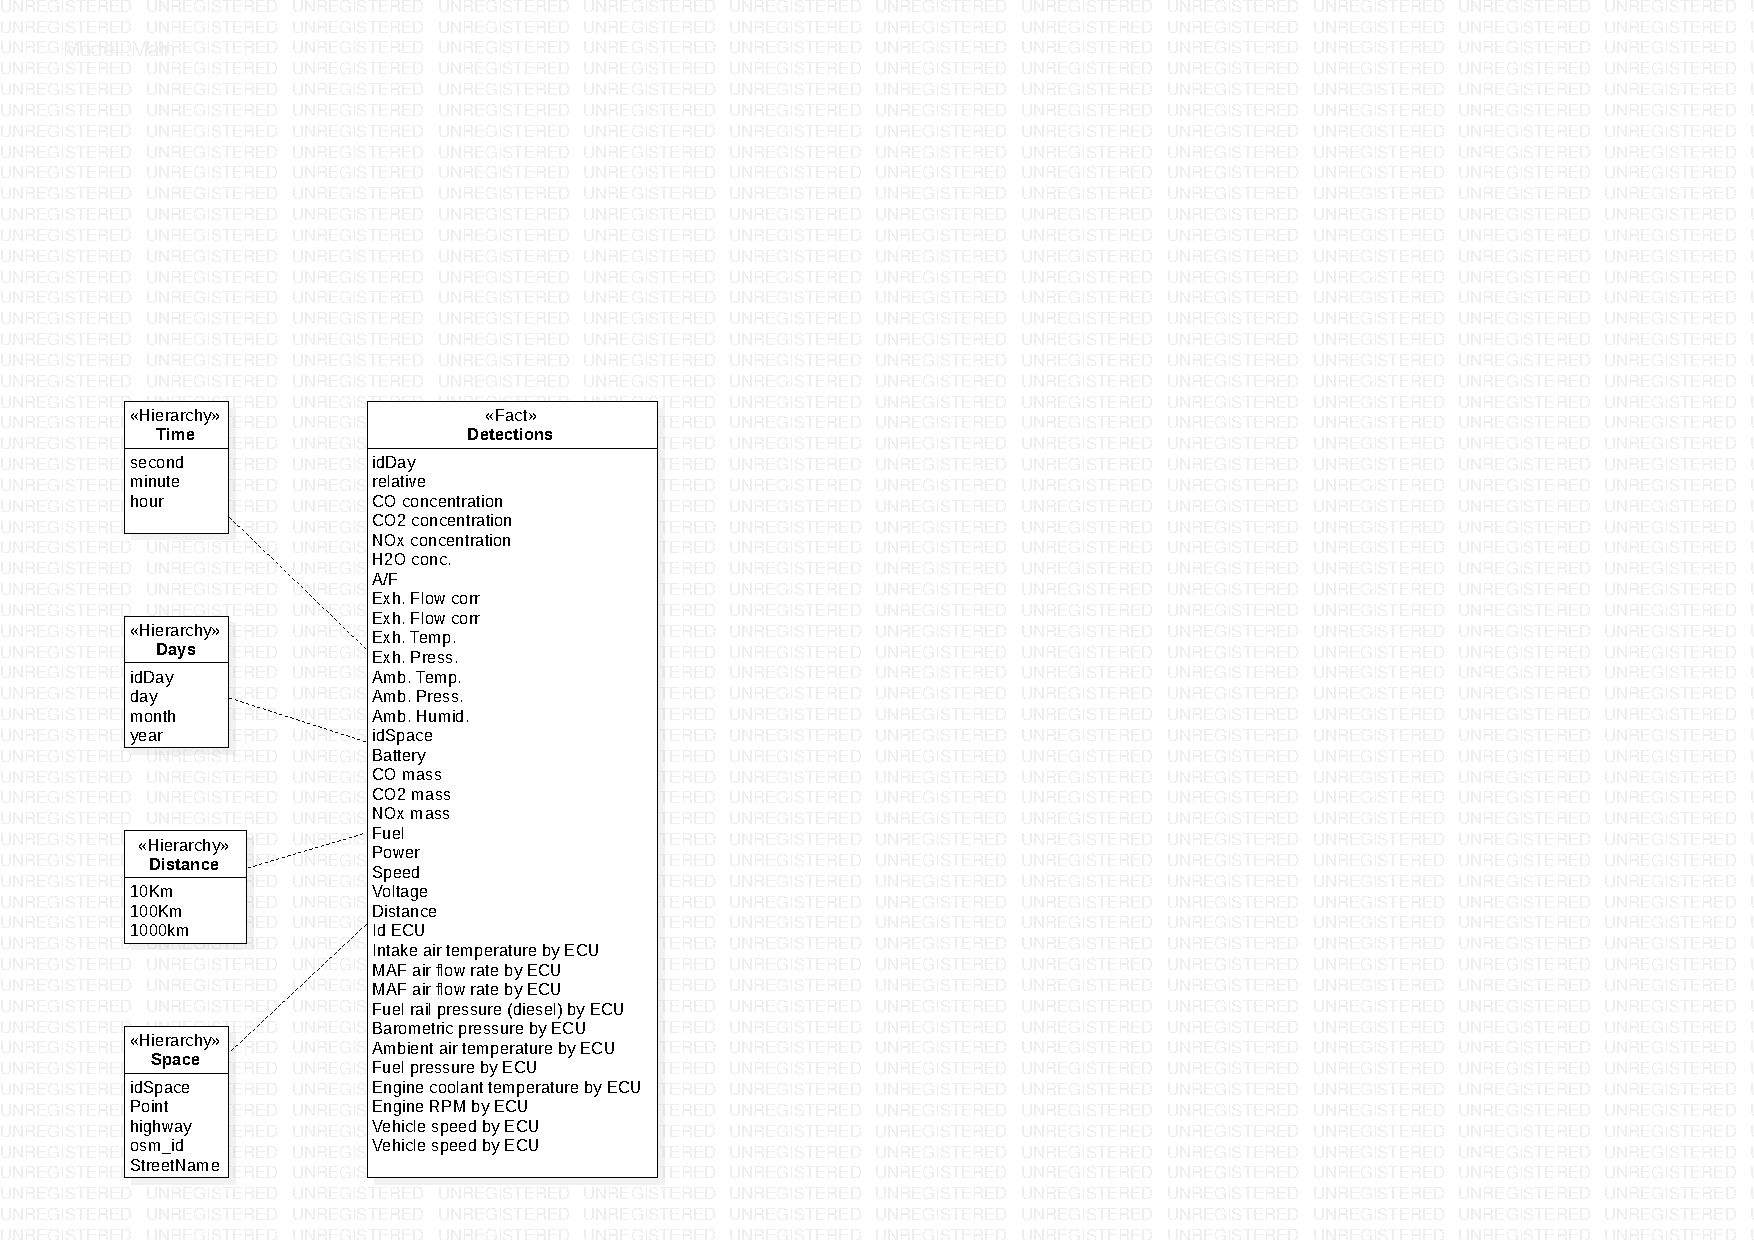
\includepdf[pages=-]{ClassDiagram.pdf}
 \title{\textbf{Query 1}}\\
Somma dei profitti ricavati per ogni combinazione [Product id- Discount].
 \begin{center}
 	\begin{table}[h!]
 	\begin{tabular}{|l|l|l|}
 		\hline
 		Product Name  & Discount & Profit \\ \hline
 		IPHONEX  & 20\% & 1000\EUR \\ \hline
 		IPHONEX  & 30\% & 3000\EUR \\ \hline
 		IPHONEX & 40\% & 2000\EUR \\ \hline
 	\end{tabular}
 \end{table}
 \end{center}

\title{\textbf{Query 2}}\\
Numero ordinato in modo decrescente dei resi effettuati per categoria di prodotto per anno.
\begin{center}
	\begin{table}[h!]
		\begin{tabular}{|l|l|l|}
			\hline
			Year & Sub-Category & Returned \\ \hline
			2018 & Chairs        & 300      \\ \hline
			2018 & Telephony    & 200      \\ \hline
			2017 & Tablets       & 400      \\ \hline
			2017 & ...          & ...      \\ \hline
			2016 & ...          & ...      \\ \hline
		\end{tabular}
	\end{table}
\end{center}
\title{\textbf{Query 3}}\\
Si raggruppa per anno e per stato ordinando in maniera decrescente i profitti relativi a quell'anno e a quello stato.
	\begin{table}[h!]
	\begin{tabular}{|l|l|l|}
		\hline
		Year & State   & Profit \\ \hline
		2018 & Italy  & 4000\EUR   \\ \hline
		2018 & France & 3000\EUR   \\ \hline
		...  & ...     & ...    \\ \hline
		2017 & ...     & ...    \\ \hline
	\end{tabular}
\end{table}
\newpage
\title{\textbf{Query 4}}\\
Si raggruppa per tipologia di cliente (Segment) e per modalità di spedizione si contano il numero di ordini.
	\begin{table}[h!]
	\begin{tabular}{|l|l|l|}
		\hline
		Segment     & Ship\_Mode & Orders \\ \hline
		Home Office & First      & 15     \\ \hline
		Home Office & Second     & 20     \\ \hline
		Consumer    & First      & 30     \\ \hline
		Consumer    & Second     & 40     \\ \hline
	\end{tabular}
\end{table}

\title{\textbf{Query 5}}\\
Per ogni anno la differenza tra i prezzi di vendita e i profitti (spese sostenute).
\begin{table}[h!]
	\begin{tabular}{|l|l|}
		\hline
		Year & Expenses (Sales -Profit) \\ \hline
		2018 & 3000000\EUR                  \\ \hline
		2017 & 2000000\EUR                  \\ \hline
		2016 & 3000000\EUR                  \\ \hline
		2015 & 100000\EUR                   \\ \hline
	\end{tabular}
\end{table}

\title{\textbf{Query 6}}\\
Per stato e per anno calcolo i soldi persi con gli sconti (Sales*Discount).
\begin{table}[h!]
	\begin{tabular}{|l|l|l|}
		\hline
		State         & Year & Economic losses( Sales*Discount) \\ \hline
		Italy         & 2018 & 50000\EUR                            \\ \hline
		Italy         & 2017 & 40000\EUR                            \\ \hline
		Italy         & 2016 & 30000\EUR                            \\ \hline
		United States & 2018 & 70000\EUR                            \\ \hline
		United States & 2017 & 60000\EUR                            \\ \hline
	\end{tabular}
\end{table}

\title{\textbf{Query 7}}\\
Per ogni prodotto/sottocategoria/categoria calcolo la media dei prezzi di vendita (eventualmente deviazione standard).
\begin{table}[h!]
	\begin{tabular}{|l|l|l|l|l|}
		\cline{1-2} \cline{4-5}
		Product     & AVG(Prices) &  & Sub-Category & AVG(Prices) \\ \cline{1-2} \cline{4-5} 
		IPHONEX     & 1000\EUR        &  & TELEPHONY    & 750\EUR         \\ \cline{1-2} \cline{4-5} 
		IPHONE7PLUS & 700\EUR         &  & COMPUTERS    & 800\EUR         \\ \cline{1-2} \cline{4-5} 
		IPHONE6     & 600\EUR         &  & TABLETS      & 500\EUR         \\ \cline{1-2} \cline{4-5} 
	\end{tabular}
\end{table}
\begin{table}[h!]
	\begin{tabular}{|l|l|}
		\hline
		Category        & AVG(Prices) \\ \hline
		FURNITURE       & 1300\EUR        \\ \hline
		TECHNOLOGY      & 1000\EUR        \\ \hline
		OFFICE SUPPLIES & 40\EUR          \\ \hline
	\end{tabular}
\end{table}

\title{\textbf{Query 8}}\\
Per mese/trimestre/anno la somma dei profitti.
\begin{table}[h!]
	\begin{tabular}{|l|l|l|l|l|l|l|l|}
		\cline{1-2} \cline{4-5} \cline{7-8}
		Month & Profits &  & Trimester   & Profits &  & Year & Profits   \\ \cline{1-2} \cline{4-5} \cline{7-8} 
		5/18  & -2000\EUR   &  & Fourth-2018 & 200000\EUR  &  & 2018 & 300000000\EUR \\ \cline{1-2} \cline{4-5} \cline{7-8} 
		6/18  & 300\EUR     &  & Third-2018  & 30029\EUR  &  & 2017 & 400000000\EUR \\ \cline{1-2} \cline{4-5} \cline{7-8} 
	\end{tabular}
\end{table}
\end{document}
